\documentclass[12pt,a4paper]{article}
\usepackage[T1]{fontenc}
\usepackage[utf8]{inputenc}
\renewcommand{\familydefault}{\sfdefault}
\usepackage{graphicx}
\usepackage{verbatim}
\usepackage{float}
\usepackage{tikz}
\usepackage{pgfplots}
\usepackage{listings}
\usepackage{datetime2}
\usepackage{booktabs}
\pgfplotsset{compat=1.16}
\restylefloat{table}
\graphicspath{{Images/}}


\AtBeginDocument{\let\today\DTMNow}
\author{Vili Lipo, 014814253}
\title{Compilers Project 2020: Mini-pl interpreter documentation}
\begin{document}
\maketitle
\newpage

\section{General view of the application}
The goal of this project was to write an interpreter for 
Mini-pl programming language. The default implementation language
for the project was C\#, but I chose to use Python, because
I am not familiar with C\#. Even though I used Python, I tried
to follow the models and patterns given in the course lectures 
as best I could. The source code for this project should be 
understandable to all who have knowledge of the common patterns
and techniques used in compilers.

In the source code of the project there are few comments, as I tried to write
the code itself in a way that is easy to read. I did not feel the need to state
the obvious twice, once in code and the second time as a comment.
Unnecessarily repeating what the code does in comments is an anti-pattern that
has no place in my projects.

\subsection{Architecture}
\begin{figure}[t]\label{big_uml}
  \caption{UML diagram of the interpreter architecture}
  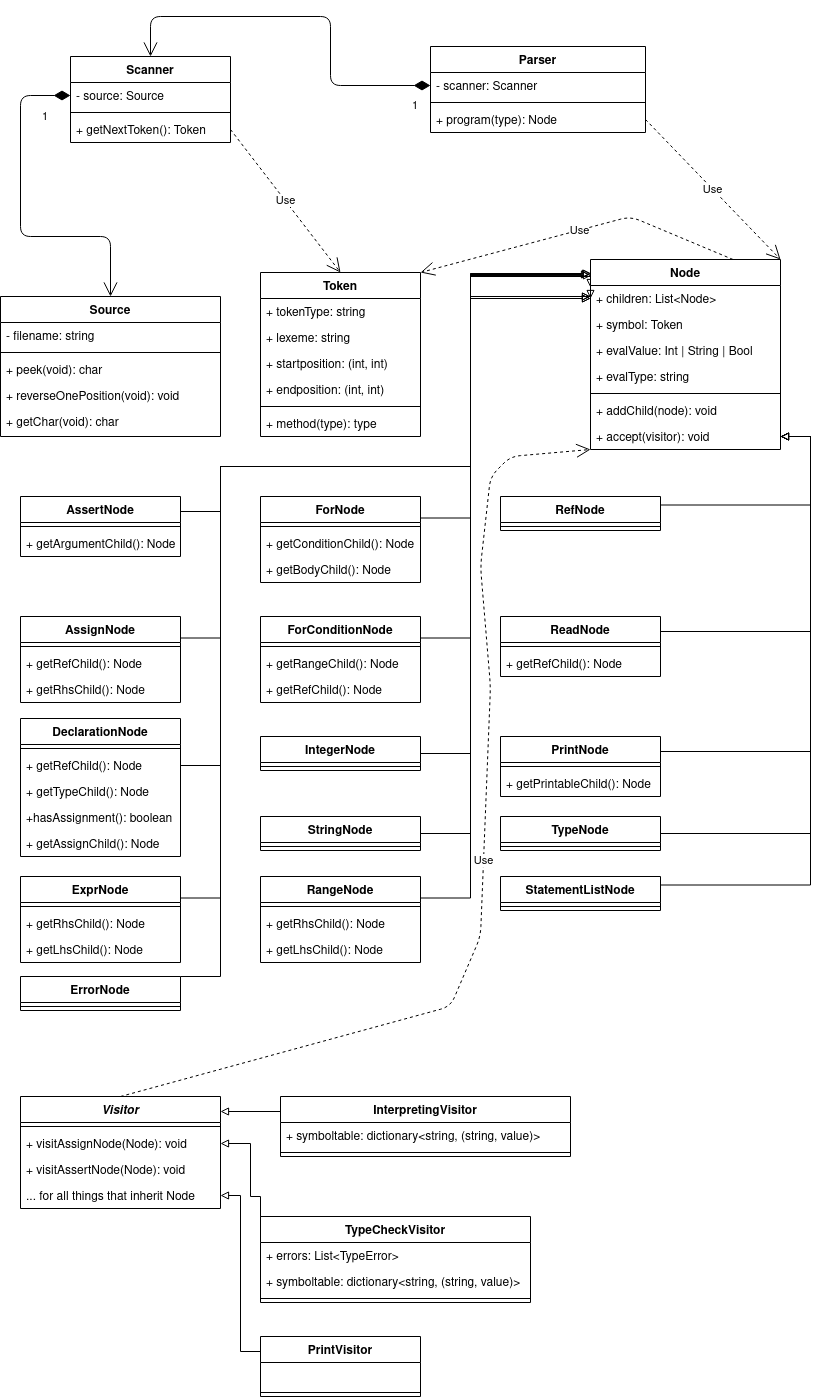
\includegraphics[scale=0.4]{reportImages/interpreter.png}
\end{figure}
The architecture of my implementation of Mini-pl interpreter
follows closely the pipeline pattern presented on the lectures.
The interpreter uses multi-pass construction, as all
parsing is done before semantical analysis, and all semantical
analysis is done before the interpreting. Although scanning
is driven by the parser, like in single pass compilers.

Overall architecture of the interpreter can be observed in figure~\ref{big_uml}.
At the lowest level we have the class Source, that is responsible
for reading a source file and giving characters from it one by one.

This is given as a constructor parameter to the class Scanner following
the dependency injection pattern. Scanner
does the lexical analysis of characters, and forms tokens out
of them. The Scanner consists of a collection of routines that
try to form a token by iterating the source. When a next
token is asked from the scanner it screens out whitespace and
comments and then it iterates through these
routines until one of them returns a valid token. If no
valid token is produced the scanner returns an error token.

When the source reaches the end-of-file, the scanner produces
end of file token.

The parser is a recursive descent parser that asks for the tokens
one by one from the scanner. Every non-terminal construct in the language has
an own method for parsing it. These methods produce abstract syntax 
tree nodes. 
The parser tries to parse new statements until the scanner produces
end of file token.

An abstract syntax tree produced by the parser
is first decorated by the TypeCheckVisitor, that
checks for semantical errors and creates a symbol table
based on variable declarations.

Symbol table created by TypeCheckVisitor is then used by
InterpretingVisitor that interprets the source file.
InterpretingVisitor further decorates the abstract 
syntax tree by setting evaluation values to the nodes,
as it goes through the program.



\subsection{Testing}

The classes Source, Scanner and Parser have quite comprehensive
unit tests written to test their core functionality. Those
can be found in the '/tests' folder. The tests for
InterpretingVisitor and TypeCheckVisitor are more in 
the integration test category.

I have taken care in 
designing these test cases and at least the tests for the
InterpretingVisitor and TypeCheckVisitor are worth to 
take look at. The Mini-pl code lines run on these tests
should give a good idea of the capabilities of this
interpreter.

Also, the `tests/test.minipl' includes all the examples given
in the language specification.
The tests contain cases for producing correct error messages.
I included a code coverage report of the unit testing as
Figure~\ref{codecov}. Total code coverage of my tests cases
is 95\%, which includes the most important corner cases
and edge behaviour in addition to normal happy path tests.


\begin{figure}\label{codecov}
  \caption{Unit and integration test code coverage}
  \begin{verbatim}
Name                                 Stmts   Miss  Cover
--------------------------------------------------------
interpreter/__init__.py                  0      0   100%
interpreter/ast.py                     179     13    93%
interpreter/interpretingvisitor.py     124      8    94%
interpreter/parser.py                  213     16    92%
interpreter/printvisitor.py             49      2    96%
interpreter/scanner.py                 153      3    98%
interpreter/source.py                   40      7    82%
interpreter/typecheckvisitor.py        157      5    97%
interpreter/visitor.py                  47     15    68%
tests/__init__.py                        0      0   100%
tests/testInterpretingVisitor.py        70      0   100%
tests/testParser.py                    160      0   100%
tests/testPrintVisitor.py               13      0   100%
tests/testScanner.py                   123      1    99%
tests/testSource.py                     23      1    96%
tests/testTypeCheckVisitor.py          131      1    99%
--------------------------------------------------------
TOTAL                                 1482     72    95%
  \end{verbatim}
\end{figure}

\subsection{Shortcomings}

The interpreter is mostly fully featured. 
The scanner supports only a limited set of escape characters that are
tabs, newlines, escape character and the quotation mark. This could
be quite easily expanded. 

The parser is bit lacking
in the error handling part, as in most of the statements, if a 
necessary token is missing the parsing of that statement will fail,
and the exception handler will try to parse a new statement all together.
This could be fixed by adding more detailed error handling to the
different statement variant methods in the Parser class. That would
make the code messier in the other hand, so I decided against it.

The Source class does not use any form of fancy buffering. It just reads
the whole file to a list of strings in its constructor. I did not think
that any buffering of source was justified as most of the programs 
that would be written using Mini-pl are short. Even in very powerful
languages most code style guides prefer files under five hundred lines with
a line length under 100 characters. Any modern computer is able to hold
5000 characters in its memory with no issues.

The visitor pattern is a bit ugly to implement in Python,
as it is not possible to overload methods by parameter types.
Despite this I think that I managed to write it in quite
readable fashion.

\subsection{Running the program}

On Linux-machines running this program should be very straight forward.
Open the directory where the archive was unzipped in a terminal.
Then move to the src directory and run
`python3 main.py  examples/tree.minipl'
to execute the example tree drawing program.
On some Linux distributions, Mac, or Windows the default Python may be the version 3,
and then you can omit the 3 from python3.
There is no additional external dependencies in running the program,
everything should be included in the python standard library.
I was able to run the program on the CS department remote shell
with no issues using the above command. Unit tests also worked
with the command `python3 -m unittest discover tests'
Generating the code coverage report would require installing 
additional python3 packages on Ubuntu 16.04 so I included it in the 
report as Figure~\ref{codecov}.


\section{Specifying the interpretation}

\subsection{Mini-PL token patterns}
The token patterns can be observed in figure~\ref{token_patterns}
\begin{figure}\label{token_patterns}
  \caption{Mini-PL token patterns}
  \begin{verbatim}
  <integer> ::= <digit>*
  <string_literal> = "<alnum>*"
  <identifier> = ([a-z] | [A-Z])([a-z] | [A-Z] | _ | [0-9])*
  <range> ::= \.\.
  <keyword> ::= var | for | end | in | do | read 
  <keyword> ::=  print | int | string | bool | assert
  <operator> ::= + | - | / | * | & | !
  \end{verbatim}
\end{figure}

\subsection{Context-free grammar}
The modified context-free grammar for Mini-pl can be seen in figure~\ref{cfg}
\begin{figure}\label{cfg}
  \caption{Modified LL (1) grammar for Mini-pl}
  \begin{verbatim}
  <prog> ::= <stmnts>
  <stmts> ::= <stmnt> ";" <stmnts>
  <stmnts> ::= <epsilon>
  <stmnt> ::= "var" <identifier> : <type> <assign_value>
  <stmnt> ::= <identifier> ":=" <expr>
  <stmnt> ::= "for" <identifier> "in" <expr> .. <expr> "do" <stmnts> end for
  <stmnt> ::= "read" <identifier> 
  <stmnt> ::=  "print" <expr>
  <stmnt> ::= "assert" ( <expr> )
  <assign_value> = := <expr>| <epsilon>
  <expr> ::= <opnd> <op> <opnd>
  <expr> ::= <unary_op> <opnd>
  <opnd> ::= <integer>
  <opnd> ::= <string_literal>
  <opnd> ::= <identifier>
  <opnd> ::= ( <expr> )
  <type> ::= "int"
  <type> ::= "string"
  <type> ::= "bool"

  \end{verbatim}
\end{figure}

\subsection{Abstract syntax tree}
The abstract syntax tree used in the interpreter, uses the composite pattern and visitor
pattern is used to manipulate the tree. 

The abstract syntax tree consists of Nodes. For each meaningful part of the
Mini-pl language I have created a subclass that inherits Node class. These
classes are listed in the figure~\ref{big_uml}. These classes are used with the
visitor pattern to do semantic analysis and interpreting.

The different classes inheriting Node class are very similar. They mostly 
differ in that some have special accessors for meaningful children nodes, like
ExprNode has methods getRhsChild, and getLhsChild.

The different visitors in this interpreter inherit the abstract class Visitor.
These objects have distinct methods for visiting all of the different nodes.

\subsection{Error Handling}

When the scanner encounters an error it sends an error token to the parser.

The parser uses context sensitive lookahead with exception driven error
handling to recover from syntax errors. Because of the way how the error
handling is written statements that are not able to be parsed will not show up
in the AST built by the parser, as the statement routine sees that there is
another symbol next, that is in its first set.

Semantic errors are discovered by TypeCheckVisitor.
These errors are printed to the user and prevent the interpreting process.
Semantic errors include usage of undeclared variables, declaring declared variables,
assigning to a wrong type, using mismatched types in expressions and assigning
to a loop variable inside a loop.

\subsection{Semantics of Mini-pl}

I have adjusted the semantics of Mini-pl a bit. In the specification
it seems that the loop variable should be one over the upper limit of the 
specified range. In my implementation when the loop ends, the loop variable
is the upper limit of the range. In essence my range is a open interval.

For the read command I decided that the strings can be a whole line,
not just a one word. It just is more flexible that way.

As for variable default values I have chosen 0 for integer, empty string for string, and 
false for boolean.

\section{Work hour log}
\begin{center}
  \begin{tabular}{l l l}
    \bottomrule
    Date & Duration & Task \\
    2.3 & 2h & Creating class Source \\
    \bottomrule
    3.3 & 1h & Initial testing of Source \\
    \bottomrule
    4.3 & 3h & Creating Scanner \\
    \bottomrule
    5.3 & 2h & Initial testing of Scanner \\
    \bottomrule
    9.3 & 1h & Creating recursive parser \\
    \bottomrule
    9.3 & 2h & Creating AST \\
    \bottomrule
    10.3 & 1h & Fixing source and scanner \\
    \bottomrule
    10.3 & 3h & Creating AST \\
    \bottomrule
    11.3 & 4h & Writing visitor abstract class and printvisitor \\
    \bottomrule
    13.3 & 6h & Writing TypeCheckVisitor and InterpretingVisitor \\
    \bottomrule
    16.3 & 3h & Finishing InterpretingVisitor and adding a launcher \\
    \bottomrule
    17.3 & 3h & Error handling in parsing \\
    \bottomrule
    17.3 & 2h & Testing. \\
    \bottomrule
    18.3 & 3h & Testing and bugfixing and adding missing features \\
    \bottomrule
    18.3 & 1h & Starting report. \\
    \bottomrule
    19.3 & 3h & Testing and bugfixing and adding missing features \\
    \bottomrule
    20.3 & 5h & Testing and bugfixing and adding missing features \\
    \bottomrule
    21.3 & 4h & Writing report and validating requirements \\
    Total & 49h & Total \\
  \end{tabular}

\end{center}



\end{document}
